\documentclass[10pt,a4paper]{article}
\usepackage[latin1]{inputenc}
\usepackage{graphicx}
\usepackage[finnish,english]{babel}
\usepackage{mathrsfs,amsfonts,amsmath,amssymb}
\usepackage[center]{lc2005}
\usepackage{fancyhdr}
\usepackage{palatino}

% Fancyheader on paketti yl�- ja alatunnisteiden muuttamiseen:
\pagestyle{fancy}
\renewcommand{\sectionmark}[1]{\markright{\thesection.\ #1}}
\lhead{\scshape \nouppercase{\rightmark}}
\chead{}
\rhead{\thepage}
\lfoot{} \cfoot{} \rfoot{}
\renewcommand{\headrulewidth}{0pt} 

 

\begin{document}

\section{Funktioteoriaa}
 
\selectlanguage{finnish}

\subsection{Aluksi}

Funktioteorian\footnote{Tunnetaan my�s kompleksianalyysin�}
sovellusaloja ovat useimmat matemaattisen analyysin alat, esimerkiksi

\begin{itemize}
\item differentiaaliyht�l�t, funktionaalianalyysi, harmoninen analyysi,
\item lukuteoria, algebra, matriisiteoria,
\item fysiikassa s�hk�oppi ja erikoisfunktiot ja
\item teknillisiss� tieteiss� elektroniikka, signaalink�sittely sek�
\item automaatio- ja s��t�tekniikka.
\end{itemize}


\subsection{Historiaa}

Funktioteorian kehitykseen vaikuttivat muiden muassa Euler, Cauchy,
Riemann, Weierstrass, Klein, Poincare ja Ahlfors (kuva \ref{hahmoja}).
Suomalaisia vaikuttajia olivat E. Lindel�f, R.  Nevanlinna, L. Alfors
ja O.  Lehto.  Funktioteorian nykyisi� tutkimuskohteita ovat
esimerkiksi \emph{kompleksi dynamiikka}, \emph{M�bius--kuvausten
  diskreetit ryhm�t} ja \emph{kvasikonformikuvaukset}.

\begin{figure}[!htbp]
\begin{center}
\hfill
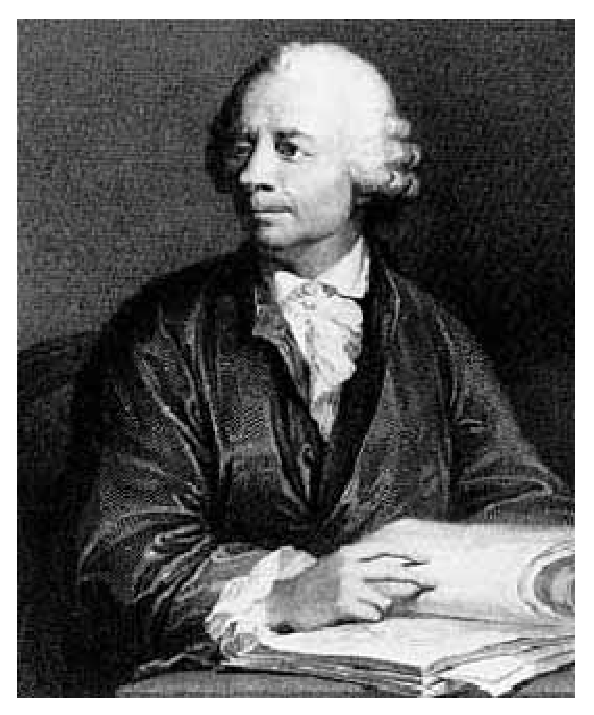
\includegraphics[width=0.2\textwidth]{Euler_8}\hfill
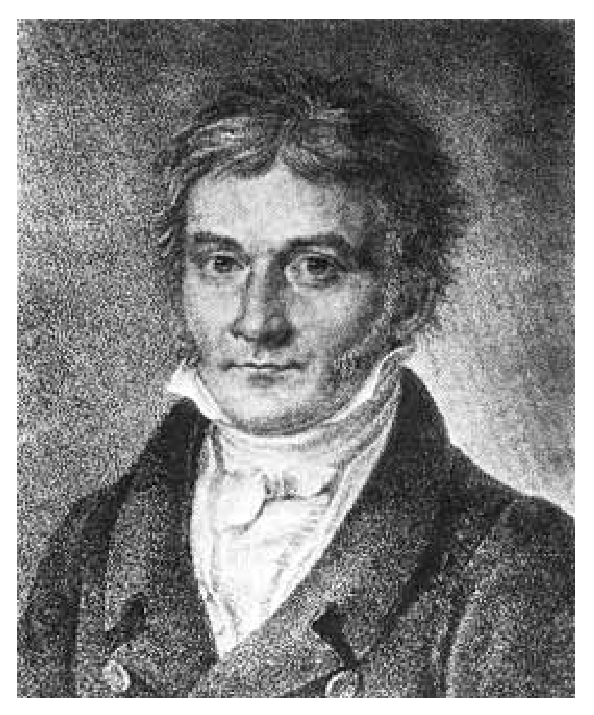
\includegraphics[width=0.2\textwidth]{Gauss_1828}\hfill
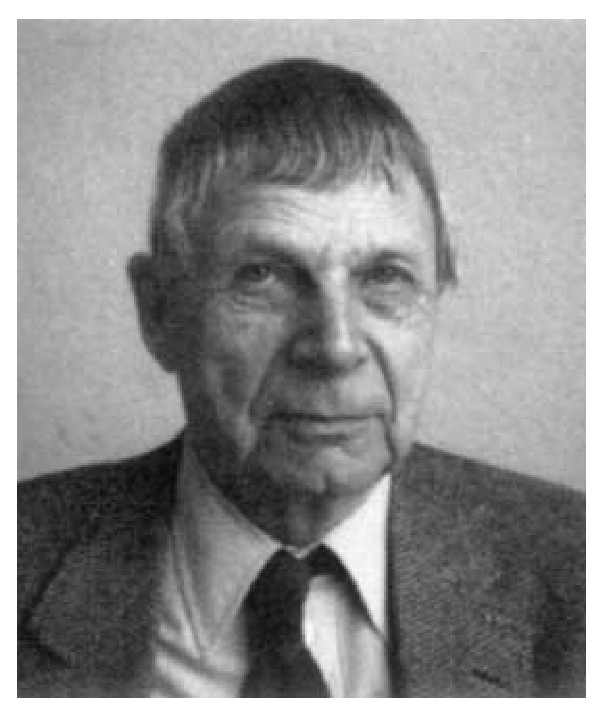
\includegraphics[width=0.2\textwidth]{Ahlfors_2}
\hfill\mbox{}
\caption{Leonhard Euler (1707 Basel, Sveitsi -- 1783
  Pietari, Ven�j�); Johann Carl Friedrich Gauss (1777 Brunswick, Saksa
  -- 1855 G�ttingen, Saksa); Lars Valerian Ahlfors (1907 Helsinki,
  Suomi -- 1996 Pittsfield, Massachusetts, USA)}
\label{hahmoja}
\end{center}
\end{figure}


Esimerkki kompleksidynamiikasta:

Etsit��n yht�l�n $f ( z ) = z^3 - 1$=0 ratkaisu Newtonin iteraartioilla
(newtonin iteraatiokaava on
\[ z_{n + 1} := z_n - \frac{f ( z_n )}{f' ( z_n )} \]
skalaarifunktioille). Mill� alkuarvolla $z_0$ ratkaisut suppenevat kohti
juurta $z = 1$? N�m� alkuarvot muodostavat geometriselta rakenteeltaan
monimutkaisen joukon, fraktaalin.


\subsection{Funktioteorian perusteet}

Kompleksiluvut $\mathbb{C}$ ovat muotoa $z = ( x, y )$, eli jokainen
alkio on j�rjestetty pari. Osoittautuu, ett� t�llaiselle parille
voidaan m��ritell� plus- ja erityisesti kompleksinen \emph{kertolasku}
niin, ett� kompleksiluvut muodostavavat kunnan. Kaiken idea on
kertolaskun ominaisuus
\[ ( 0, 1 ) ( 0, 1 ) = ( - 1, 0 ), \]
jota merkit��n my�s $\sqrt{- 1} = i$. T�h�n p��st��n merkitsem�ll�
vastaavuudet
\[ ( 1, 0 ) \sim 1 \quad \text{ja} \quad ( 0, 1 ) \sim i. \]
Kompleksiluvun $z$ reaaliosa $x$ voidaan aina poimia funktiolla
${\mathrm Re} ( \cdot )$ ja imaginaariosa $y$ funktiolla ${\mathrm Im}
( \cdot )$, mik�li osia tarvitaan erikseen.


 
\end{document}
